% id: 105-14
% book: 베이직쎈 미적분1 · 06 도함수의 활용 (3)
% section: 학교 시험 기출로 실전 감각 UP!
% figure: tikz:fig-105-14
% answer: 
% answer_source: 
% variant_level: 0 (원본 전사)
% 이 파일은 build.mjs 가 items.json 에서 만든다. 고칠 때는 items.json 을 고친다.
\smash{\raisebox{1.5mm}{\dmkichul{베이직쎈 미적분1 105쪽 14번 · 서답형 · 서술형}}}
\noindent\begin{minipage}[t]{0.58\linewidth}\vspace{0pt}\raggedright 밑면의 반지름의 길이가 $10\mkern3mu \mathrm{cm}$, 높이가 $8\mkern3mu \mathrm{cm}$인 원뿔 모양의 빈 그릇에 오른쪽 그림과 같이 매초 $1\mkern3mu \mathrm{cm}$씩 수면의 높이가 올라가도록 물을 넣을 때, 다음에 답하시오.\end{minipage}\hfill\begin{minipage}[t]{0.4\linewidth}\vspace{0pt}\centering \resizebox{\ifdim\width>\linewidth\linewidth\else\width\fi}{!}{% 105-14(105쪽) — 밑면의 반지름의 길이가 10 cm, 높이가 8 cm 인 원뿔 모양의 빈 그릇에 물을 넣는 그림(수면이 올라가는 것을 화살표로 표시). 스캔 화질이 낮아 TikZ 로 다시 그림.
% 원문에 있는 것만 옮긴다: 원뿔 그릇 · 안쪽 벽 · 밑면의 반지름(10 cm)과 직각 표시 · 높이 치수 점선(8 cm) · 수면 두 자리와 올라가는 화살표. 수면 높이는 원문 그림의 비율 그대로 그려 답이 읽히지 않게 한다.
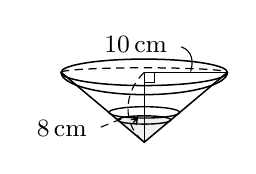
\begin{tikzpicture}[x=0.24cm, y=0.24cm, line width=0.55pt]
  % 담긴 물
  \fill[gray!12] (-1.41,1.18) arc(180:360:1.41 and 0.22) -- (0,0) -- cycle;
  \fill[gray!12] (-1.41,1.18) arc(180:0:1.41 and 0.22) -- (0,0) -- cycle;
  % 그릇
  \draw (0,3.7) ellipse (4.4 and 0.70);
  \draw (-4.4,3.7) arc(180:360:4.4 and 1.18);
  \draw[densely dashed, line width=0.45pt] (-4.4,3.7) arc(180:0:4.4 and 0.24);
  \draw (-4.4,3.7) -- (0,0) -- (4.4,3.7);
  % 높이와 밑면의 반지름
  \draw[line width=0.5pt] (0,3.7) -- (0,0);
  \draw[line width=0.5pt] (0,3.7) -- (4.4,3.7);
  \draw[line width=0.4pt] (0,3.18) -- (0.52,3.18) -- (0.52,3.7);
  % 수면
  \draw[line width=0.5pt] (0,1.58) ellipse (1.87 and 0.30);
  \draw[line width=0.5pt] (0,1.18) ellipse (1.41 and 0.22);
  \draw[->, >=stealth, line width=0.4pt] (-0.62,0.98) -- (-0.30,1.40);
  % 치수
  \draw[densely dashed, line width=0.4pt] (0,3.7) .. controls (-1.15,2.6) and (-1.15,0.9) .. (0,0);
  \draw[densely dashed, line width=0.4pt] (-2.30,0.80) -- (-1.05,1.30);
  \node[left=1.5pt, font=\small] at (-2.30,0.72) {$8\,\mathrm{cm}$};
  \draw[line width=0.4pt] (1.95,5.05) .. controls (2.55,4.85) and (2.62,4.25) .. (2.45,3.74);
  \node[left=1.5pt, font=\small] at (1.95,5.15) {$10\,\mathrm{cm}$};
\end{tikzpicture}
}\end{minipage}\par
\dmsubprob{1} $t$초 후의 수면의 높이를 $t$에 대한 식으로 나타내시오.
\dmsubprob{2} $t$초 후의 수면의 반지름의 길이를 $t$에 대한 식으로 나타내시오.
\dmsubprob{3} $4$초 후의 그릇에 담긴 물의 부피의 변화율을 구하시오.
